\documentclass[10pt]{article}

\usepackage{xifthen}% \isempty
\usepackage{stringstrings}% \substring

\usepackage{nameref}
\makeatletter
\newcommand*{\currentlabel}{\@currentlabel}
\makeatother

\usepackage{amsmath, amsthm, amssymb}
\usepackage{fullpage}
\usepackage[colorlinks=false,urlcolor=blue,pageanchor=true]{hyperref}
\usepackage{xspace}
\usepackage{graphicx}
\usepackage[normalem]{ulem}
\usepackage{enumitem}
\usepackage{adjustbox}

\newtheorem{lemma}{Lemma}
\newtheorem{definition}{Definition}
\newtheorem{theorem}{Theorem}
\newtheorem{corollary}{Corollary}
\newtheorem{claim}{Claim}

\newcommand{\E}{\operatorname{E}}
\newcommand{\giv}{\,|\,}
\newcommand{\Z}{\mathbb{Z}}
\newcommand{\Zp}{\mathbb{Z}_{\ge 0}}
\newcommand{\R}{\mathbb{R}}
\newcommand{\Rp}{\mathbb{R}_{\ge 0}}
\newcommand{\N}{\mathbb{N}}
\newcommand{\Np}{\mathbb{N}_{\ge 0}}

\newcommand{\OP}[1]{{\small\sc #1}\xspace}
\newcommand{\Insert}{\OP{Insert}}
\newcommand{\FindMin}{\OP{Find-Min}}
\newcommand{\DeleteMin}{\OP{Delete-Min}}
\newcommand{\DecreaseKey}{\OP{Decrease}}
\newcommand{\Merge}{\OP{Merge}}
\newcommand{\Cut}{\OP{Cut}}

\setlength{\parskip}{2pt}
% \setlength{\parindent}{0in}

\setlength\fboxsep{0pt}
\newlist{steps}{enumerate}{9}
\setlist[steps]{wide,label*=\arabic*.,topsep=1pt,parsep=1pt,partopsep=1pt,itemsep=0pt, labelindent=2pt}%
\setlist[steps,1]{ref=\arabic*}
\setlist[steps,2]{ref=\arabic{stepsi}.\arabic*}
\setlist[steps,3]{ref=\arabic{stepsi}.\arabic{stepsii}.\arabic*}
\setlist[steps,4]{ref=\arabic{stepsi}.\arabic{stepsii}.\arabic{stepsiii}.\arabic*}
\setlist[steps,5]{ref=\arabic{stepsi}.\arabic{stepsii}.\arabic{stepsiii}.\arabic{stepsiv}.\arabic*}
\setlist[steps,6]{ref=\arabic{stepsi}.\arabic{stepsii}.\arabic{stepsiii}.\arabic{stepsiv}.\arabic{\stepsv}.\arabic*}
\setlist[steps,7]{ref=\arabic{stepsi}.\arabic{stepsii}.\arabic{stepsiii}.\arabic{stepsiv}. \arabic{\stepsv}.\arabic{\stepsvi}.\arabic*}
\setlist[steps,8]{ref=\arabic{stepsi}.\arabic{stepsii}.\arabic{stepsiii}.\arabic{stepsiv}. \arabic{\stepsv}.\arabic{\stepsvi}.\arabic{\stepsvii}.\arabic*}
\setlist[steps,9]{ref=\arabic{stepsi}.\arabic{stepsii}.\arabic{stepsiii}.\arabic{stepsiv}. \arabic{\stepsv}.\arabic{\stepsvi}. \arabic{\stepsvii}.\arabic{\stepsviii}.\arabic*}

\newlist{asteps}{enumerate}{6}
\setlist[asteps]{wide,topsep=1pt,parsep=1pt,partopsep=1pt,itemsep=0pt, labelindent=1em}%
\setlist[asteps,1]{
  label=\alph*.,
  ref=\alph*
}
\setlist[asteps,2]{
  label=\alph{astepsi}.\arabic*.,
  ref=\alph{astepsi}.\arabic*
}
\setlist[asteps,3]{
  label=\alph{astepsi}.\arabic{astepsii}.\arabic*.,ref=\alph{astepsi}.\arabic{astepsii}.\arabic*
}
\setlist[asteps,4]{
  label=\alph{astepsi}.\arabic{astepsii}.\arabic{astepsiii}.\arabic*.,
  ref=\alph{astepsi}.\arabic{astepsii}.\arabic{astepsiii}.\arabic*
}
\setlist[asteps,5]{
  label=\alph{astepsi}.\arabic{astepsii}.\arabic{astepsiii}.\arabic{astepsiv}.\arabic*.,
  ref=\alph{astepsi}.\arabic{astepsii}.\arabic{astepsiii}.\arabic{astepsiv}.\arabic*
}
\setlist[asteps,6]{
  label=\alph{astepsi}.\arabic{astepsii}.\arabic{astepsiii}.\arabic{astepsiv}.\arabic{\astepsv}.\arabic*.,
  ref=\alph{astepsi}.\arabic{astepsii}.\arabic{astepsiii}.\arabic{astepsiv}.\arabic{\astepsv}.\arabic*
}

\newlist{problems}{enumerate}{9}
\setlist[problems]{wide, label=\textbf{Problem \arabic*},topsep=1pt,parsep=1pt,partopsep=1pt,itemsep=0pt, labelindent=0pt}%

\newcommand{\STEPS}{steps}
\newcommand{\SHIFT}{\renewcommand{\SHIFT}{\renewcommand{\STEPS}{asteps}}}

\newcommand{\maybeLabel}[1]{\ifthenelse{\isempty{#1}}{}{\label{#1}}}
\newcommand{\maybeItem}[1]{\ifthenelse{\isempty{#1}}{\item}{\item[#1]}}

\newcommand{\problem}[1][]{\maybeItem{#1}~\par}

\newenvironment{longFormProof}[1][Proof (long form).]
{\SHIFT\begin{proof}[#1]~\par\begin{\STEPS}}{\end{\STEPS}\vspace*{-1ex}\end{proof}}

\newenvironment{shortFormProof}[1][Proof (short form).]
{\SHIFT\begin{proof}[#1]}{\end{proof}}

% \makeatletter
% \newcommand{\caseitem}{\@sitem}
% \newcommand{\@sitem}{%
%   \refstepcounter{\@enumctr}%
%   \item[\textbullet~\csname label\@enumctr\endcsname]}
% \makeatother

\newcommand{\step}[1][]{\item\maybeLabel{#1}}

\newcommand{\comment}[1]{\hfill{\footnotesize\emph{#1}}}

\newcommand{\lineacross}{\par\vspace*{-0.7\baselineskip}\noindent\hrulefill\par}

\newenvironment{block}[2][]
{\step[#1]  #2 \begin{\STEPS}}{\end{\STEPS}}

\newenvironment{case}[2][]
{\step[#1] (case \currentlabel) \emph{#2}\begin{\STEPS}}{\end{\STEPS}}

\newcommand{\setHeader}{\markboth
{\footnotesize CS 145 turn-in \turnIn, \today, by \author, \SID}
{\footnotesize CS 145 turn-in \turnIn, \today, by \author, \SID}}

\newcommand{\setTurnIn}[1]{\newcommand{\turnIn}{#1}}
\newcommand{\setAuthor}[1]{\renewcommand{\author}{#1}}
\newcommand{\setSID}[1]{\newcommand{\SID}{#1}}

\pagestyle{myheadings}
\addtolength{\headsep}{0.3in}
\addtolength{\topmargin}{-0.4in}
\addtolength{\textheight}{0.4in}

%%% Local Variables:
%%% mode: latex
%%% TeX-master: "assignment-template"
%%% End:


% TODO: CHANGE NAME AND SID TO YOURS:

\setTurnIn{11}  

\setAuthor{YOUR NAME HERE}
\setSID{YOUR SID HERE}
\setHeader

\begin{document}

\begin{problems}

  %%%%%%%%%%%%%%%%%%%%%%%%%%%%%%%%%%%%%%%%%%%%%%%%%%%%%%%%%%%% 
  %%%%%%%%%%%%%%%%%%%%%%%%%%%%%%%%%%%%%%%%%%%%%%%%%%%%%%%%%%%% 

  \problem % problem 1

  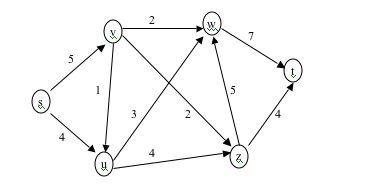
\includegraphics{graph}

  {\vskip 0.1in \noindent\bf Maximum flows:}

    We can get a maximum flow of 9 by giving the edges in the graph the following flows:\\
    $f(s, v) = 5,\\
     f(s, u) = 4,\\
     f(v, w) = 2,\\
     f(v, z) = 2,\\
     f(v, u) = 1,\\
     f(u, w) = 1,\\
     f(u, z) = 4,\\
     f(z, t) = 4,\\
     f(z, w) = 2,\\
     f(w, t) = 5\\$

  {\vskip 0.1in \noindent\bf Minimum cuts:}

    There are a few minimum cuts for this problem. You could cut the set of edges $\{(s, v), (s, u)\}$ for a cost of 9, 
        or you could cut $\{(s, u), (v, w), (v, u), (v, z)\}$ for a cost of 9.

  {\vskip 0.1in \noindent\bf Critical edges:}

    Critical edges here are all in the set $\{(s, v), (s, u), (v, w), (v, u), (v, z)\}$
  
  %%%%%%%%%%%%%%%%%%%%%%%%%%%%%%%%%%%%%%%%%%%%%%%%%%%%%%%%%%%% 
  %%%%%%%%%%%%%%%%%%%%%%%%%%%%%%%%%%%%%%%%%%%%%%%%%%%%%%%%%%%% 

  \newpage 

  \problem % problem 2

  %%%%%%%%%%%%%%%%%%%%%%%%%%%%%%%%%%%%%%%%%%%%%%%%%%%%%%%%%%%% 
  %%%%%%%%%%%%%%%%%%%%%%%%%%%%%%%%%%%%%%%%%%%%%%%%%%%%%%%%%%%% 

  \setcounter{lemma}{1}
  \begin{lemma}
    An edge $e$ is critical if and only if $f(e) = \text{cap}(e)$ in every maximum flow $f$.
  \end{lemma}

  \begin{longFormProof}

    \begin{block}[B]
      {Consider any $s$-$t$ flow network $G$ and edge $e$.

      \lineacross }
      
      \step First we will prove that, if $f(e) \ne \text{cap}(e)$ in some maximum flow $f$, then $e$ is not critical.

      \smallskip 
      
      \begin{block}[B1]
        {Assume that there exists max-flow $f$ such that $f(e) \ne \text{cap}(e)$.}

        \step Let $\epsilon = \text{cap}(e) - f(e) > 0$.  (Using here that $f(e) \le \text{cap}(e)$ and $f(e)\ne\text{cap}(e)$.)

        \step Let $G'$ be the graph obtained by reducing the capacity of $e$ by $\epsilon$.

        \step $\text{cap}(e)$ in $G'$ is greater than or equal to $f(e)$ in $G$.

        \step Therefore, the max flow, $f$ in $G$ is also feasible in $G'$.

        \step So $e$ is not critical.
      \end{block}

      \step[B2] By block~\ref{B1}, if $f(e) \ne \text{cap}(e)$ in some maximum flow $f$,
      then $e$ is not critical.

      \smallskip 

      \lineacross 

      \step Next we will prove that, if $e$ is not critical, then $f(e) \ne \text{cap}(e)$ in some maximum flow.

      \smallskip 

      \begin{block}[B3]
        {Assume that $e$ is not critical in $G$.}

        \step[S1] Let $\epsilon>0$ be such that reducing the capacity of $e$ by $\epsilon$ does not reduce the maximum flow value.  (Such an $\epsilon$ exists by the definition of ``critical'').

        \step Let $G'$ be the graph obtained by reducing the capacity of $e$ by $\epsilon$.

        \step By the definition of a critical edge, $G'$ will have the same maximum flow value as $G$.

        \step That is, the maximum flow in $G'$ could be applied to $G$ and $f(e)$ would be $\text{cap}(e) - \epsilon$.

        \step There is a max flow $f$ in $G$ with $f(e) \ne \text{cap}(e)$.
      \end{block}
      
      \step[B4] By block~\ref{B3}, if $e$ is not critical, then there exists a maximum flow $f$ in $G$
      with $f(e) \ne \text{cap}(e)$.

      \smallskip

      \lineacross 
    
      \step By lines~\ref{B2} and~\ref{B4},
      $e$ is critical if and only if $f(e) = \text{cap}(e)$ in every maximum flow $f$ in $G$.
    \end{block}

    \step By block~\ref{B},
    for any edge $e$ in any flow network,
    $e$ is critical iff $f(e) = \text{cap}(e)$ in every max flow $f$ in $G$.
  \end{longFormProof}

\end{problems}

\end{document}

%%% Local Variables:
%%% mode: latex
%%% TeX-master: t
%%% End:
